%!TEX root = ../thesis.tex
%*******************************************************************************
%******************************  5th  Chapter **********************************
%*******************************************************************************

\chapter{Experimental results}
\label{chap:xp}
% **************************** Define Graphics Path **************************
\ifpdf
    \graphicspath{{Chapter5/Figs/Raster/}{Chapter5/Figs/PDF/}{Chapter5/Figs/}}
\else
    \graphicspath{{Chapter5/Figs/Vector/}{Chapter5/Figs/}}
\fi




\section{Technical difficulties} % (fold)
\label{sec:technical_difficulties}

Where do I write about the numerous issues ?
\begin{itemize}
  \item Inferno is unstable
  \item Pivot is unstable
  \item TP requires Jacobian vector product or takes crazy amount of time to train
  \item Regressor requires slow Adam and is probably a pain to train with gaussian mixture
  \item
\end{itemize}



The benchmark is controlled with many parameters
\begin{itemize}
  \item Number of test samples
  \item Parameter of the toy model
  \item True value of the parameter of interest and nuisance parameters
  \item Sampling random seed
  \item TODO finish this list
\end{itemize}








\section{Performances on toys} % (fold)
\label{sec:performances_on_toys}

The idea is to do one subsection for one result
\begin{itemize}
  \item Result 1 : The more test samples the better the inference
  \item Result 2 : Calib > Prior as expected
  \item Result final : Who is the best ?
  \item 5. Regressor estimated variance is probably broken
\end{itemize}


Let's start with the results on the two toy problems (see \autoref{sec:toy_datasets} for details).
Toys provide a fully controled environement on various parameters of the problem to confront the proposed methods against different difficulties.
The first one is the small number of samples to do inference (\autoref{sub:performance_according_to_sample_size}).










\subsection{Performance according to sample size} % (fold)
\label{sub:performance_according_to_sample_size}

Here is summaried the performances measured according to the number of sample of the test set.

On the nominal test set (\autoref{fig:gg_baseline_nominal_n_samples_mse}) the MSE behaves as expected \ie decreases fast (probably $\frac{1}{\sqrt{N}}$) as the size of the test set increase.
Only Pivot seems to have some issues.
This indicates that all models works corectly.

\begin{figure}[ht!]
  \centering
  \begin{subfigure}[t]{0.49\linewidth}
    \includegraphics[width=\linewidth]{COMPARE/GG-prior/GradientBoostingModel/profusion_nominal_n_samples_mse.png}
    \caption{Gradient boosting}
    % \label{fig:gg-prior_GB_profusion_nominal_n_samples_mse}
  \end{subfigure}%
  \hfill
  \begin{subfigure}[t]{0.49\linewidth}
    \includegraphics[width=\linewidth]{COMPARE/GG-prior/NeuralNetClassifier/profusion_nominal_n_samples_mse.png}
    \caption{Neural network classifier}
    % \label{fig:gg-calib_best_average_errplot_mse}
  \end{subfigure}

  \begin{subfigure}[t]{0.49\linewidth}
    \includegraphics[width=\linewidth]{COMPARE/GG-prior/DataAugmentation/profusion_nominal_n_samples_mse.png}
    \caption{Data augmentation}
    % \label{fig:gg-prior_GB_profusion_nominal_n_samples_mse}
  \end{subfigure}%
  \hfill
  \begin{subfigure}[t]{0.49\linewidth}
    \includegraphics[width=\linewidth]{COMPARE/GG-prior/TangentPropClassifier/profusion_nominal_n_samples_mse.png}
    \caption{Tangent Prop}
    % \label{fig:gg-calib_best_average_errplot_mse}
  \end{subfigure}

  \begin{subfigure}[t]{0.49\linewidth}
    \includegraphics[width=\linewidth]{COMPARE/GG-prior/Inferno/profusion_nominal_n_samples_mse.png}
    \caption{Inferno}
    % \label{fig:gg-prior_GB_profusion_nominal_n_samples_mse}
  \end{subfigure}%
  \hfill
  \begin{subfigure}[t]{0.49\linewidth}
    \includegraphics[width=\linewidth]{COMPARE/GG-prior/PivotClassifier/profusion_nominal_n_samples_mse.png}
    \caption{Pivot classifier}
    % \label{fig:gg-calib_best_average_errplot_mse}
  \end{subfigure}

  \begin{subfigure}[t]{0.49\linewidth}
    \includegraphics[width=\linewidth]{COMPARE/GG-prior-plus/Regressor/profusion_nominal_n_samples_mse.png}
    \caption{Regressor}
    % \label{fig:gg-prior_GB_profusion_nominal_n_samples_mse}
  \end{subfigure}%
  \hfill
  \begin{subfigure}[t]{0.49\linewidth}
    \includegraphics[width=\linewidth]{COMPARE/GG-marginal/Regressor/profusion_nominal_n_samples_mse.png}
    \caption{Regressor marginal}
    % \label{fig:gg-calib_best_average_errplot_mse}
  \end{subfigure}


  \caption{MSE of $\hmu$ according to the number of samples on nominal data only. Each curve correspond to a model with a specific set of hyper-parameter.}
  \label{fig:gg_baseline_nominal_n_samples_mse}
\end{figure}


This is less obvious on the non nominal data (\autoref{fig:gg_baseline_n_samples_mse}).

The 1D toy problem (named GG) is asymetric in $\alpha$.
Indeed increasing $\alpha$ will move appart the center of the signal and the background distribution.
On the other hand when comparing the nominal distribution and the one with a smaller $\alpha$ the signal spike will go under the background blanquet.
With a small amount on signal and a small $\alpha$ the signal spike could be confused with a flucuation making inference harder.
This is why blue curves $\alpha=0.8$ are way above the $\alpha=1.2$ green curves in most models.

Inferno and the marginal Regressor are not affected by this assymetry.
Maybe those 2 neural networks are measuring $\alpha$ then correcting it ?
The marginal Regressor is expected to do so at least.


\begin{figure}[ht!]
  \centering
  \begin{subfigure}[t]{0.49\linewidth}
    \includegraphics[width=\linewidth]{COMPARE/GG-prior/GradientBoostingModel/profusion_n_samples_mse.png}
    \caption{Gradient boosting}
    % \label{fig:gg-prior_GB_profusion_n_samples_mse}
  \end{subfigure}%
  \hfill
  \begin{subfigure}[t]{0.49\linewidth}
    \includegraphics[width=\linewidth]{COMPARE/GG-prior/NeuralNetClassifier/profusion_n_samples_mse.png}
    \caption{Neural network classifier}
    % \label{fig:gg-calib_best_average_errplot_mse}
  \end{subfigure}

  \begin{subfigure}[t]{0.49\linewidth}
    \includegraphics[width=\linewidth]{COMPARE/GG-prior/DataAugmentation/profusion_n_samples_mse.png}
    \caption{Data augmentation}
    % \label{fig:gg-prior_GB_profusion_n_samples_mse}
  \end{subfigure}%
  \hfill
  \begin{subfigure}[t]{0.49\linewidth}
    \includegraphics[width=\linewidth]{COMPARE/GG-prior/TangentPropClassifier/profusion_n_samples_mse.png}
    \caption{Tangent Prop}
    % \label{fig:gg-calib_best_average_errplot_mse}
  \end{subfigure}

  \begin{subfigure}[t]{0.49\linewidth}
    \includegraphics[width=\linewidth]{COMPARE/GG-prior/Inferno/profusion_n_samples_mse.png}
    \caption{Inferno}
    % \label{fig:gg-prior_GB_profusion_n_samples_mse}
  \end{subfigure}%
  \hfill
  \begin{subfigure}[t]{0.49\linewidth}
    \includegraphics[width=\linewidth]{COMPARE/GG-prior/PivotClassifier/profusion_n_samples_mse.png}
    \caption{Pivot classifier}
    % \label{fig:gg-calib_best_average_errplot_mse}
  \end{subfigure}

  \begin{subfigure}[t]{0.49\linewidth}
    \includegraphics[width=\linewidth]{COMPARE/GG-prior/Regressor/profusion_n_samples_mse.png}
    \caption{Regressor}
    % \label{fig:gg-prior_GB_profusion_n_samples_mse}
  \end{subfigure}%
  \hfill
  \begin{subfigure}[t]{0.49\linewidth}
    \includegraphics[width=\linewidth]{COMPARE/GG-marginal/Regressor/profusion_n_samples_mse.png}
    \caption{Regressor marginal}
    % \label{fig:gg-calib_best_average_errplot_mse}
  \end{subfigure}

  \caption{MSE of $\hmu$ according to the number of samples. Each curve correspond to a model with a specific set of hyper-parameter and a value of $\alpha^\star$. The colors correspond to the values of $\alpha^\star$. Here only the value of $\mu^\star$ is kept as nominal.}
  \label{fig:gg_baseline_n_samples_mse}
\end{figure}



\victor{TODO : Evolution de la variance stat et syst en fonction de N\_samples.}







\subsection{Calibration influence} % (fold)
\label{sub:calibration_influence}


\victor{TODO : Le terme CALIBRATION est probablement pas cool. Il lui faudrait donner un autre nom. On fait pas ça dans une région de controle. Et on perd l'indépendance de la calibe avec $\mu$ donc c'est pas de la calibration. Mais c'est pas forcément une mauvaise idée !}

In this benchmark two way of calibrating the data is used.
\begin{enumerate}
  \item Trust a given prior
  \item Infer the nuisance parameter distribution using a regressor
\end{enumerate}

Here we show that the later improves significantly the performances of all methods.
Indeed using only a poorly informed prior leads the baseline to a biased estimator as shown in \autoref{fig:gg_baseline_compare_calib_estimator} for a neural net classifier.
It is clear that the estimation depends on $\alpha^\star$ and is biased if $\alpha^\star$ is not the nominal value.
\victor{TODO : GB \&PIVOT \& TP \& REG show the same behaviour. INFERNO is not affected. DA is more robust.}

Using the given data to improve calibration leads to an unbiased estimator.
\victor{TODO : Someone may argue that it is because my prior calibration is bad. But my simulator cannot do better...}



\begin{figure}[ht!]
  \centering
  \begin{subfigure}[t]{0.49\linewidth}
    \includegraphics[width=\linewidth]{COMPARE/GG-prior/GradientBoostingModel/profusion_true_mu_target_mean.png}
    \caption{Prior calibration}
    % \label{fig:gg-prior_GB_profusion_n_samples_mse}
  \end{subfigure}%
  \hfill
  \begin{subfigure}[t]{0.49\linewidth}
    \includegraphics[width=\linewidth]{COMPARE/GG-calib/GradientBoostingModel/profusion_true_mu_target_mean.png}
    \caption{Using data in calibration to infer $\alpha$}
    % \label{fig:gg-calib_best_average_errplot_mse}
  \end{subfigure}

  \begin{subfigure}[t]{0.49\linewidth}
    \includegraphics[width=\linewidth]{COMPARE/GG-prior/NeuralNetClassifier/profusion_true_mu_target_mean.png}
    \caption{Prior calibration}
    % \label{fig:gg-prior_GB_profusion_n_samples_mse}
  \end{subfigure}%
  \hfill
  \begin{subfigure}[t]{0.49\linewidth}
    \includegraphics[width=\linewidth]{COMPARE/GG-calib/NeuralNetClassifier/profusion_true_mu_target_mean.png}
    \caption{Using data in calibration to infer $\alpha$}
    % \label{fig:gg-calib_best_average_errplot_mse}
  \end{subfigure}

  \caption{Many estimations of the \textbf{baselines models}. Each point is colored according to the value of $\alpha^\star$. The x-axis is representing the value of $\mu^\star$. Each point is the average of the estimated interest parameter ($\hmu$) over cross validation of one neural network classifier (one hyper-parameter set).}
  \label{fig:gg_baseline_compare_calib_estimator}
\end{figure}

\begin{figure}[ht!]
  \centering
  \begin{subfigure}[t]{0.49\linewidth}
    \includegraphics[width=\linewidth]{COMPARE/GG-prior/DataAugmentation/profusion_true_mu_target_mean.png}
    \caption{Prior calibration}
    % \label{fig:gg-prior_GB_profusion_n_samples_mse}
  \end{subfigure}%
  \hfill
  \begin{subfigure}[t]{0.49\linewidth}
    \includegraphics[width=\linewidth]{COMPARE/GG-calib/DataAugmentation/profusion_true_mu_target_mean.png}
    \caption{Using data in calibration to infer $\alpha$}
    % \label{fig:gg-calib_best_average_errplot_mse}
  \end{subfigure}

  \begin{subfigure}[t]{0.49\linewidth}
    \includegraphics[width=\linewidth]{COMPARE/GG-prior/TangentPropClassifier/profusion_true_mu_target_mean.png}
    \caption{Prior calibration}
    % \label{fig:gg-prior_GB_profusion_n_samples_mse}
  \end{subfigure}%
  \hfill
  \begin{subfigure}[t]{0.49\linewidth}
    \includegraphics[width=\linewidth]{COMPARE/GG-calib/TangentPropClassifier/profusion_true_mu_target_mean.png}
    \caption{Using data in calibration to infer $\alpha$}
    % \label{fig:gg-calib_best_average_errplot_mse}
  \end{subfigure}

  \begin{subfigure}[t]{0.49\linewidth}
    \includegraphics[width=\linewidth]{COMPARE/GG-prior/PivotClassifier/profusion_true_mu_target_mean.png}
    \caption{Prior calibration}
    % \label{fig:gg-prior_GB_profusion_n_samples_mse}
  \end{subfigure}%
  \hfill
  \begin{subfigure}[t]{0.49\linewidth}
    \includegraphics[width=\linewidth]{COMPARE/GG-calib/PivotClassifier/profusion_true_mu_target_mean.png}
    \caption{Using data in calibration to infer $\alpha$}
    % \label{fig:gg-calib_best_average_errplot_mse}
  \end{subfigure}

  \begin{subfigure}[t]{0.49\linewidth}
    \includegraphics[width=\linewidth]{COMPARE/GG-prior/Inferno/profusion_true_mu_target_mean.png}
    \caption{Prior calibration}
    % \label{fig:gg-prior_GB_profusion_n_samples_mse}
  \end{subfigure}%
  \hfill
  \begin{subfigure}[t]{0.49\linewidth}
    \includegraphics[width=\linewidth]{COMPARE/GG-calib/Inferno/profusion_true_mu_target_mean.png}
    \caption{Using data in calibration to infer $\alpha$}
    % \label{fig:gg-calib_best_average_errplot_mse}
  \end{subfigure}

  \caption{Many estimations of the \textbf{systematic aware models}. Each point is colored according to the value of $\alpha^\star$. The x-axis is representing the value of $\mu^\star$. Each point is the average of the estimated interest parameter ($\hmu$) over cross validation of one neural network classifier (one hyper-parameter set).}
  \label{fig:gg_syst_aware_compare_calib_estimator}
\end{figure}

\begin{figure}[ht!]
  \centering
  \begin{subfigure}[t]{0.49\linewidth}
    \includegraphics[width=\linewidth]{COMPARE/GG-prior/Regressor/profusion_true_mu_target_mean.png}
    \caption{Prior calibration}
    % \label{fig:gg-prior_GB_profusion_n_samples_mse}
  \end{subfigure}%
  \hfill
  \begin{subfigure}[t]{0.49\linewidth}
    \includegraphics[width=\linewidth]{COMPARE/GG-calib/Regressor/profusion_true_mu_target_mean.png}
    \caption{Using data in calibration to infer $\alpha$}
    % \label{fig:gg-calib_best_average_errplot_mse}
  \end{subfigure}

  \begin{subfigure}[t]{0.49\linewidth}
    \includegraphics[width=\linewidth]{COMPARE/GG-marginal/Regressor/profusion_true_mu_target_mean.png}
    \caption{Marginal}
    % \label{fig:gg-prior_GB_profusion_n_samples_mse}
  \end{subfigure}%

  \caption{Many estimations of the \textbf{regressor models}. Each point is colored according to the value of $\alpha^\star$. The x-axis is representing the value of $\mu^\star$. Each point is the average of the estimated interest parameter ($\hmu$) over cross validation of one neural network classifier (one hyper-parameter set).}
  \label{fig:gg_regressor_compare_calib_estimator}
\end{figure}



The 1D toy problem is asymetric by definition which leads to an asymetry in performances when using the prior calibration.
This asymetry tends to disapear when the calibration is done on the data (see \autoref{fig:gg_baseline_compare_calib_n_samples_mse}).


\begin{figure}[ht!]
  \centering
  \begin{subfigure}[t]{0.49\linewidth}
    \includegraphics[width=\linewidth]{COMPARE/GG-prior/NeuralNetClassifier/profusion_n_samples_mse.png}
    \caption{Calibration with a prior on $\alpha$}
    % \label{fig:gg-prior_GB_profusion_nominal_n_samples_mse}
  \end{subfigure}%
  \hfill
  \begin{subfigure}[t]{0.49\linewidth}
    \includegraphics[width=\linewidth]{COMPARE/GG-calib/NeuralNetClassifier/profusion_n_samples_mse.png}
    \caption{Using data in calibration to infer $\alpha$}
    % \label{fig:gg-calib_best_average_errplot_mse}
  \end{subfigure}
  \caption{MSE of $\hmu$ according to the number of samples. Each curve correspond to a model with a specific set of hyper-parameter and a value of $\alpha^\star$. The colors correspond to the values of $\alpha^\star$. Here only the value of $\mu^\star$ is kept as nominal.}
  \label{fig:gg_baseline_compare_calib_n_samples_mse}
\end{figure}









\subsection{Compare methods} % (fold)
\label{sub:compare_methods}


The good news is that systematic aware learning and the direct approach is giving better results that the baseline (\autoref{fig:compare_gg_best_mse}).

\begin{figure}[ht!]
  \centering
  \begin{subfigure}[t]{0.49\linewidth}
    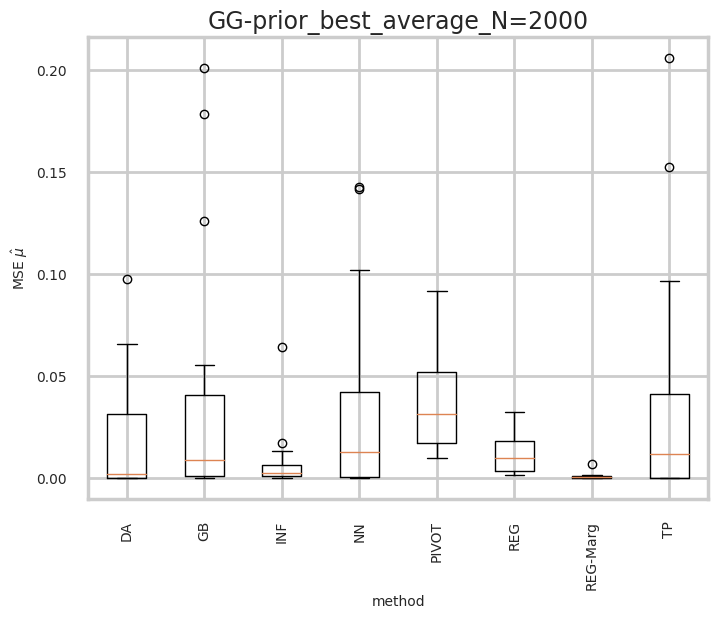
\includegraphics[width=\linewidth]{COMPARE/GG-prior/BEST_MSE/GG-prior_best_average_N=2000-boxplot_mse.png}
    \caption{Boxplot of MSE on Prior}
    % \label{fig:gg-prior_best_average_boxplot_mse}
  \end{subfigure}%
  \hfill
  \begin{subfigure}[t]{0.49\linewidth}
    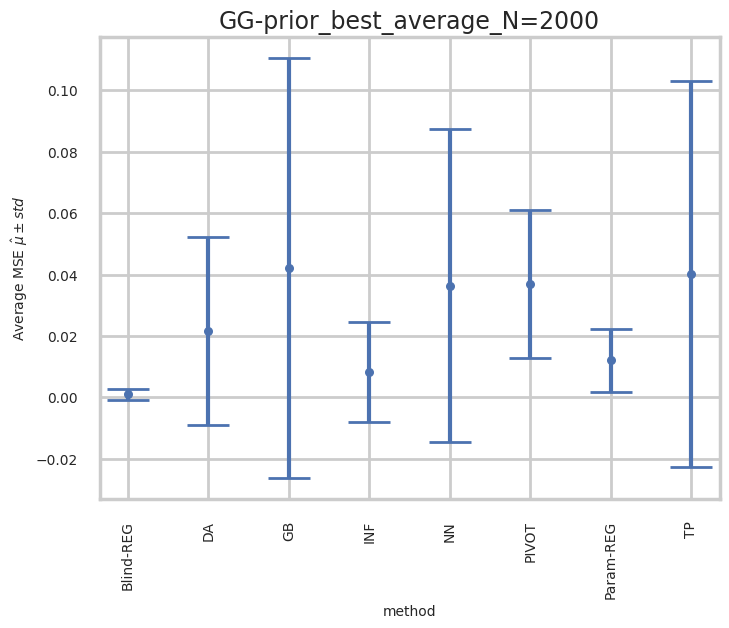
\includegraphics[width=\linewidth]{COMPARE/GG-prior/BEST_MSE/GG-prior_best_average_N=2000-errplot_mse.png}
    \caption{Average MSE $\pm$ variance on Prior}
    % \label{fig:gg-prior_best_average_errplot_mse}
  \end{subfigure}

  \begin{subfigure}[t]{0.49\linewidth}
    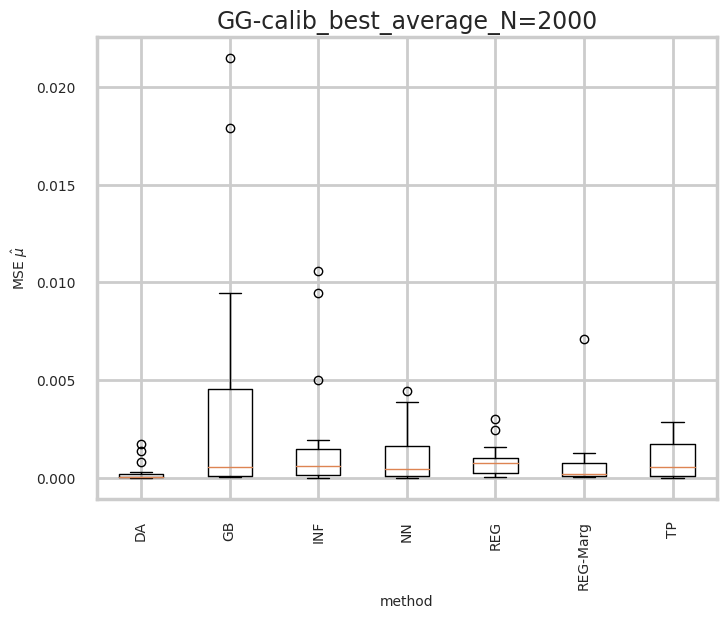
\includegraphics[width=\linewidth]{COMPARE/GG-calib/BEST_MSE/GG-calib_best_average_N=2000-boxplot_mse.png}
    \caption{Boxplot of MSE on Calibrated GG}
    % \label{fig:gg-prior_best_average_boxplot_mse}
  \end{subfigure}%
  \hfill
  \begin{subfigure}[t]{0.49\linewidth}
    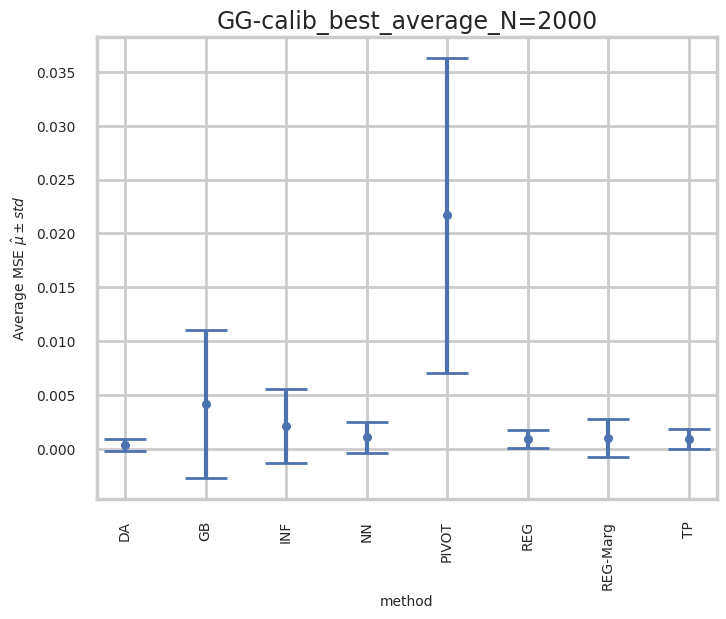
\includegraphics[width=\linewidth]{COMPARE/GG-calib/BEST_MSE/GG-calib_best_average_N=2000-errplot_mse.png}
    \caption{Average MSE $\pm$ variance on Calibrated GG}
    % \label{fig:gg-calib_best_average_errplot_mse}
  \end{subfigure}

  \caption{MSE on GG with 2000 test samples. Distribution according to $\mu^\star$ and $\alpha^\star$. The chosen model (hyper-parameter set) for each method is the model with the best average MSE.}
  \label{fig:compare_gg_best_mse}
\end{figure}

Reg-Marginal is very good on the 1D toy problem which may be explained by the simplicity of the problem.
The average of the only observable $x$ is linearly connected to the parameter of interest (see \autoref{fig:gg_mean_link}).
The only extra work the marginal regressor has to do is to infer $\alpha$ to adjust itsinference which is also very simple in this toy.

\begin{figure}[ht!]
  \centering
  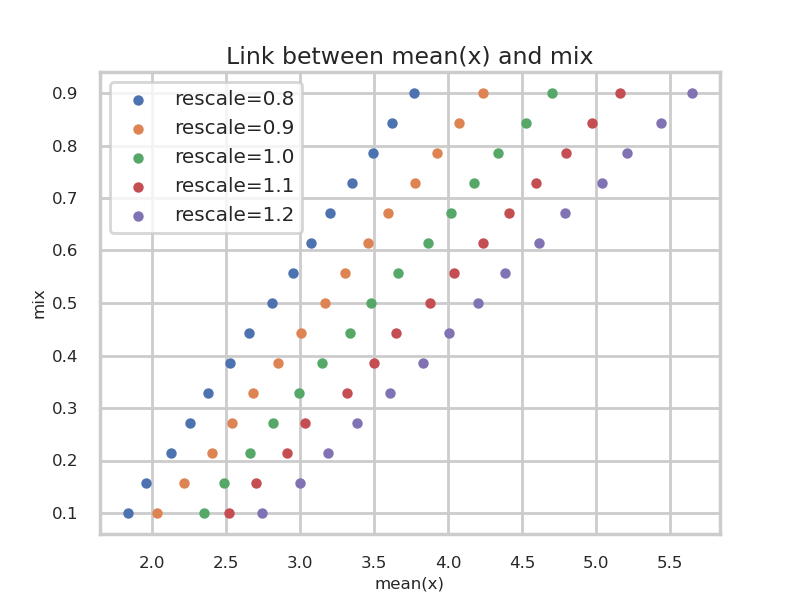
\includegraphics[width=0.49\linewidth]{GG/mean_link.png}
  \caption{link between $\mu^\star$ and the average of $x$ on GG toy problem}
  \label{fig:gg_mean_link}
\end{figure}


Inferno is doing very well including on the Prior calibration.

Tangent propagation is failing to learn a robust distribution.
This is expected as the only feature $x$ is both very correlated to the parameter of interest but also to the nuisance parameter.
Making the classification good and independant from $\alpha$ at the sample level is not possible.

Data augmentation is very good !
Data augmentation is learning to be less confident about the classification which spread the score distribution of the signals.
This spreading leads to splitting signal events into 2 bins instead on one (see \autoref{fig:gg_prior_distrib_summaries}).
\textbf{But how is it helping inference ???}

\begin{figure}[ht!]
  \centering
  \begin{subfigure}[t]{0.49\linewidth}
    \includegraphics[width=\linewidth]{GG-prior/NeuralNetClassifier/valid_distrib.png}
    \caption{NN score distribution}
    % \label{fig:gg-prior_best_average_boxplot_mse}
  \end{subfigure}%
  \hfill
  \begin{subfigure}[t]{0.49\linewidth}
    \includegraphics[width=\linewidth]{GG-prior/DataAugmentation/valid_distrib.png}
    \caption{DA score distribution}
    % \label{fig:gg-prior_best_average_errplot_mse}
  \end{subfigure}

  \begin{subfigure}[t]{0.49\linewidth}
    \includegraphics[width=\linewidth]{GG-prior/NeuralNetClassifier/valid_summaries.png}
    \caption{NN summaries}
    % \label{fig:gg-prior_best_average_boxplot_mse}
  \end{subfigure}%
  \hfill
  \begin{subfigure}[t]{0.49\linewidth}
    \includegraphics[width=\linewidth]{GG-prior/DataAugmentation/valid_summaries.png}
    \caption{DA summaries}
    % \label{fig:gg-calib_best_average_errplot_mse}
  \end{subfigure}

  \caption{Score distribution and bin counts for NN classifier and data augmentation}
  \label{fig:gg_prior_distrib_summaries}
\end{figure}



\victor{TODO : Compare methods also according to number of samples ! REG and DA are very good with small test size}
The regressor and data augmentation are very good with small test size \autoref{fig:compare_gg_best_mse50_samples} even when using only prior calibration.

\begin{figure}[ht!]
  \centering
  \begin{subfigure}[t]{0.49\linewidth}
    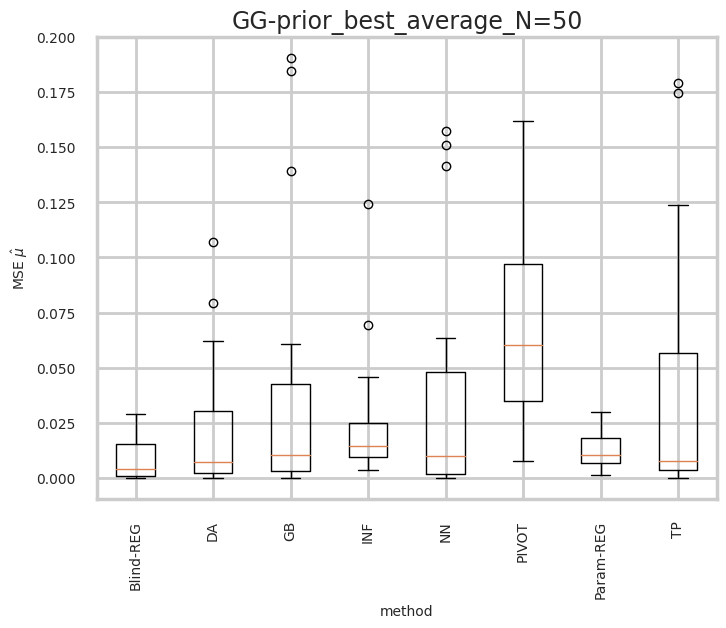
\includegraphics[width=\linewidth]{COMPARE/GG-prior/BEST_MSE/GG-prior_best_average_N=50-boxplot_mse.png}
    \caption{Boxplot of MSE on Prior}
    % \label{fig:gg-prior_best_average_boxplot_mse}
  \end{subfigure}%
  \hfill
  \begin{subfigure}[t]{0.49\linewidth}
    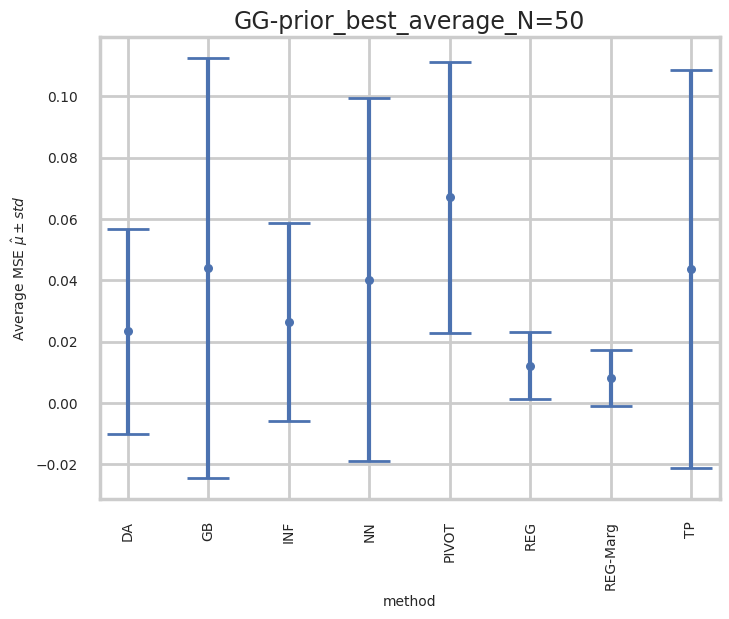
\includegraphics[width=\linewidth]{COMPARE/GG-prior/BEST_MSE/GG-prior_best_average_N=50-errplot_mse.png}
    \caption{Average MSE $\pm$ variance on Prior}
    % \label{fig:gg-prior_best_average_errplot_mse}
  \end{subfigure}

  \begin{subfigure}[t]{0.49\linewidth}
    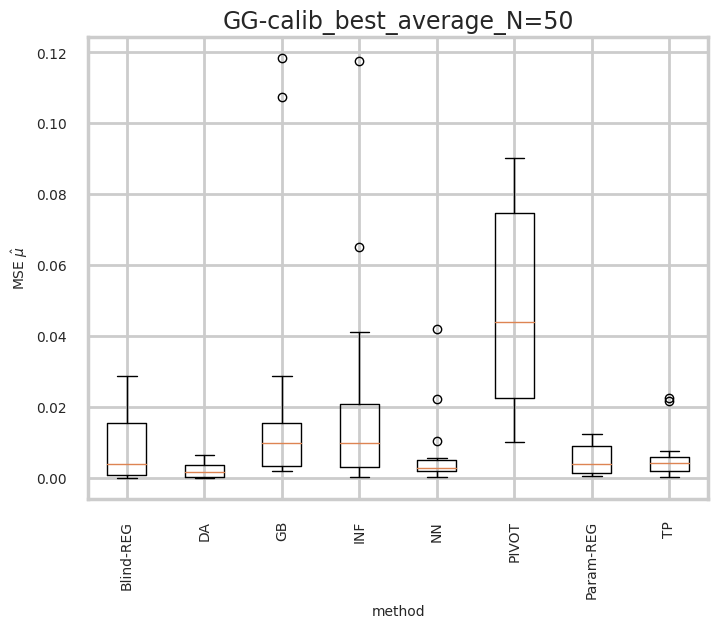
\includegraphics[width=\linewidth]{COMPARE/GG-calib/BEST_MSE/GG-calib_best_average_N=50-boxplot_mse.png}
    \caption{Boxplot of MSE on Calibrated GG}
    % \label{fig:gg-prior_best_average_boxplot_mse}
  \end{subfigure}%
  \hfill
  \begin{subfigure}[t]{0.49\linewidth}
    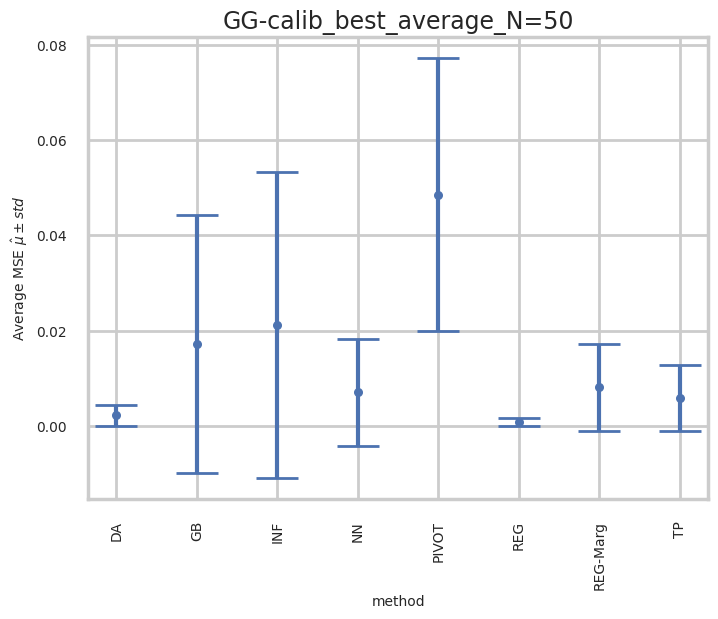
\includegraphics[width=\linewidth]{COMPARE/GG-calib/BEST_MSE/GG-calib_best_average_N=50-errplot_mse.png}
    \caption{Average MSE $\pm$ variance on Calibrated GG}
    % \label{fig:gg-calib_best_average_errplot_mse_}
  \end{subfigure}

  \caption{MSE on GG with 50 test samples. Distribution according to $\mu^\star$ and $\alpha^\star$. The chosen model (hyper-parameter set) for each method is the model with the best average MSE.}
  \label{fig:compare_gg_best_mse50_samples}
\end{figure}


\victor{TODO : ajouter les méthodes qui utilisent la vrai likelihood et Bayes.}




\subsection{V stat and V syst} % (fold)
\label{sub:v_stat_and_v_syst}

Pivot and Inferno are clearly tradding $V_{stat}$ and $V_{syst}$.
They show high values of $V_{stat}$ and very low values of $V_{syst}$ compared to the other methods.

It results is very good inference for inferno but pivot is show poor MSE performance ... why ?



Inferno is bad at v stat but always the best at v syst !



\begin{figure}[ht!]
  \centering
  \begin{subfigure}[t]{0.49\linewidth}
    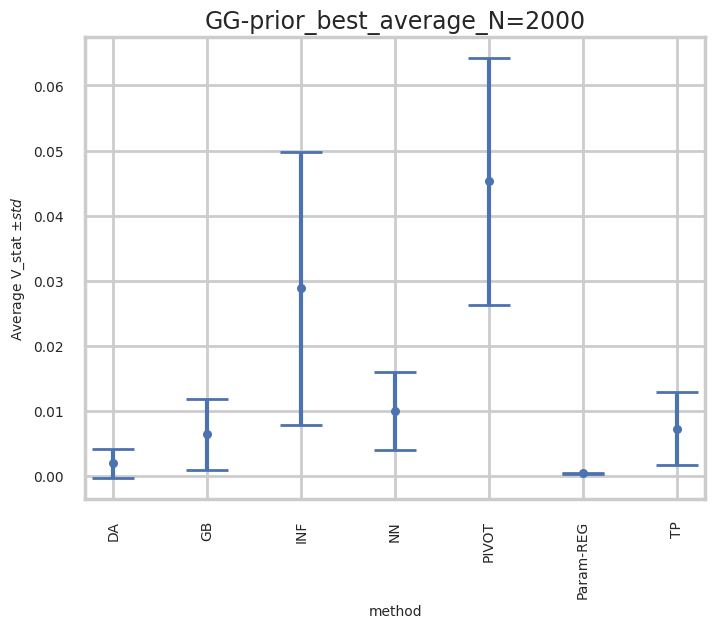
\includegraphics[width=\linewidth]{COMPARE/GG-prior/BEST_MSE/GG-prior_best_average_N=2000-errplot_v_stat.png}
    \caption{$V_{stat}$}
    % \label{fig:gg-prior_GB_profusion_nominal_n_samples_mse}
  \end{subfigure}%
  \hfill
  \begin{subfigure}[t]{0.49\linewidth}
    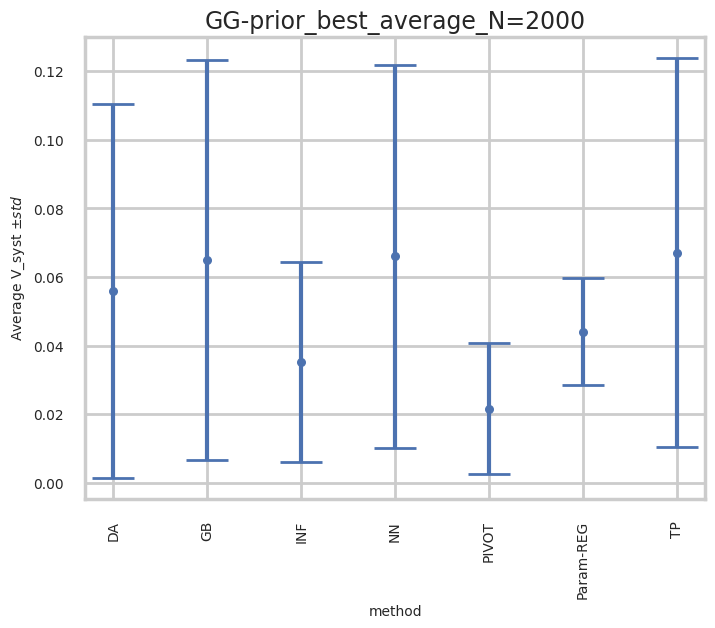
\includegraphics[width=\linewidth]{COMPARE/GG-prior/BEST_MSE/GG-prior_best_average_N=2000-errplot_v_syst.png}
    \caption{$V_{syst}$}
    % \label{fig:gg-calib_best_average_errplot_mse}
  \end{subfigure}
  \caption{Vstat and Vsyst for the best models (TODO more details)}
  \label{fig:compare_gg_prior_best_mse_v_stat_syst}
\end{figure}

















\clearpage
\victor{TODO remove temporary clearpage}

\section{Real data} % (fold)
\label{sec:real_data}


\victor{Find out why this is does not work : \url{https://arxiv.org/pdf/1909.03081.pdf} ??}
\victor{La simulation est trop précise. cf resultat sur l'impossibilité de séparer les domaines créé}








\subsection{Nothing beats the baseline} % (fold)
\label{sub:nothing_beats_the_baseline}

\content{Show results on Higgs}







\subsection{Impossible to separate between domains} % (fold)
\label{sub:impossible_to_separate_between_domains}

\content{Show results of classifier trying to separate events between "extreme" values of nuisance params}









\subsection{Results with or without calibration} % (fold)
\label{sub:results_with_or_without_calibration}

\content{Compare results with or without using the current data in the calibration}







\subsection{Too rare signals} % (fold)
\label{sub:too_rare_signals}


\content{Explain and show that the issue comes from the imbalance between signals and backgrounds}

The scatter plot properties is much more dependent to noise or nuisance parameters than to the parameter of interest.







1. XP Toy 1D
2. XP Toy 3D
3. XP Broken 1D 3D
4. Higgs
5. Repaired Higgs
